\documentclass{article}
\usepackage[utf8]{inputenc}
\usepackage{graphicx, color}
\usepackage[brazil]{babel}
\usepackage{minted}
\usepackage{url}
\usepackage[top = 3cm, botton =3cm, right=3cm, left=3cm ]{geometry}

\title{A2 - Trabalho equivalente à A1 de Análise Exploratória e Visualização de Dados}
\author{Profº: Asla Medeiros\\
Tutor: Antonio Neto\\
Aluna: Nicole dos Santos de Souza}
\date{Outubro, 2022}

\begin{document}

\maketitle
\newpage
\tableofcontents
\newpage

\section{Etapa 1 - pesquisa}
Observação: Os códigos correspondentes às funções utilizadas estão em anexo ao documento.

\subsection{ Principais medidas de Centralidade}
 Dentre todas as informações presentes em um conjunto de dados, podemos retirar valores que representem, de algum modo, todo o conjunto. Esses valores são denominados “Medidas de Tendência Central" ou "Medidas de Centralidade”. As mais recorrentes são a Média Aritmética, a Moda e a Mediana.
 \subsubsection{Média Aritmética}
A média aritmética é uma medida de tendência que se aplica somente a variáveis numéricas e consiste na seguinte fórmula:

$$\=x = \frac{x_1 + x_2 + \cdots + x_n}{n} $$

onde $x_1, x_2, x_3, \cdots, x_n$ é um conjunto de observações de média aritmética $\=x$.

\subsubsection{Moda}
É a medida de centralidade que corresponde ao valor observado com mais frequência em um conjunto de dados, aplicada tanto a variáveis quantitativas quanto qualitativas. Quando um conjunto não apresenta moda, dizemos que ele é amodal. Caso exista uma moda (e apenas uma) denominamos o conjunto de Unimodal. Quando há duas modas (dois valores possuem a mesma frequência e ela é a maior do conjunto) denominamos o conjunto de bimodal e assim sucessivamente.

\subsubsection{Mediana}
Chama-se de mediana de um conjunto de dados ao valor que tem a seguinte propriedade: a
metade das observações são maiores ou iguais, e a outra metade é menor ou igual a esse valor. Em
termos intuitivos, a mediana é o que indica exatamente o valor central de um conjunto quando organizados em ordem crescente ou decrescente. Quando a quantidade de dados é par, a mediana consiste na média aritmética entre os dois valores centrais.

\subsection{Principais medidas de Dispersão}
As medidas de dispersão têm como finalidade avaliar quão espalhadas estão as observações de
uma variável em torno dos seus valores centrais. Aqui estarão descritas as seguintes medidas: o desvio-padrão, a variância e os quartis. 

\subsubsection{Desvio padrão}
A medida de dispersão mais comumente utilizada é o desvio padrão, que está representado na fórmula abaixo:

$$ \sigma = \sqrt{\frac{(x_1 - \=x)^2 + (x_2 - \=x)^2 + \dots + (x_n - \=x)^2}{n}} $$

onde $x_1, x_2, x_3, \cdots, x_n$ é um conjunto de observações de desvio padrão $\sigma$.

Um baixo desvio padrão indica que os pontos dos dados tendem a
estar próximos da média ou do valor esperado.
 Um alto desvio padrão indica que os pontos dos dados estão
espalhados por uma ampla gama de valores.

\subsubsection{Variância}
A interpretação da variância é a mesma que a do desvio padrão, está relacionada a quão espelhados os dados estão em torno da média. A variância, nada mais é, do que $\sigma^2$, ou seja, $(desvio\_padrão)^2$. Sendo assim, sua fórmula é:

$$ \sigma^2 = \frac{(x_1 - \=x)^2 + (x_2 - \=x)^2 + \dots + (x_n - \=x)^2}{n} $$

\subsubsection{Quartis}
Outra forma de tentar avaliar o grau de dispersão de uma variável consiste em obter quais valores
em que certos números de frequência acumulada são atingidos. Em geral, consideramos os valores 0,
25\%, 50\%, 75\% e 100\%, que correspondem aos chamados quartis da variável. Note que os quartis
correspondentes a 0, 50\% e 100\% são, respectivamente, o valor mínimo, o valor máximo e a
mediana das observações. 
Há um tipo de gráfico diretamente associado com os quartis, chamado de {\it boxplot} ou {\it diagrama de caixas}. Ele é muito utilizado para entender o grau de dispersão de um conjunto de dados. \\

\newpage
Sua representação está descrita abaixo:

\begin{figure}[!h]
\centering
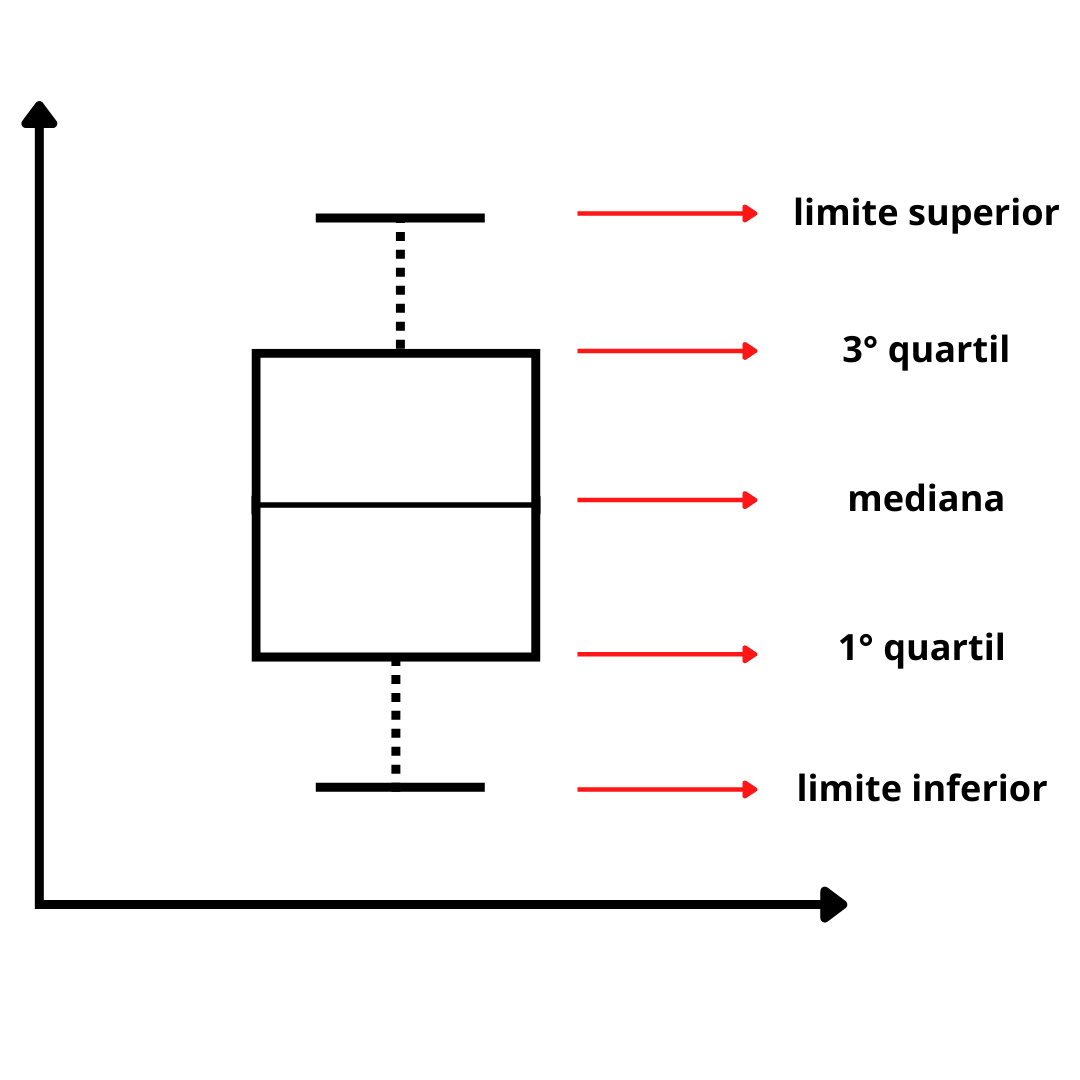
\includegraphics[width=8cm]{images/boxplot.png}
\end{figure}

\subsection{Principais medidas de Associação}
Para propósitos de tomada de decisão, é útil identificar se existe uma
associação linear entre duas variáveis ou entre mais de duas variáveis e, se
apropriado, quantificar essa associação. Uma
medida estatística  bastante útil para verificar a
associação entre dois conjuntos de dados é chamada de coeficiente de correlação ou grau de associação. 

\subsubsection{Coeficiente de Correlação}
Se temos um conjunto de observações $x_1, x_2, \dots, x_n$, definimos o coeficiente de correlação
como:

$$\rho = \frac{\sum_{i=1}^{n}(x_i - \=x)(y_i - \=y)}{\sqrt{\sum_{i=1}^{n}(x_i-\=x)^2}\sqrt{\sum_{i=1}^{n}(y_i-\=y)^2}}$$

Observa-se que as quantidades no denominador são os desvios-padrão de cada variável. Os valores do coeficiente de correlação variam entre −1 e 1. Além disso, esses valores
extremos só ocorrem quando existem {\it a} e {\it b}, tais que $y_i = ax_i + b$ para $i = 1, 2, \cdots, n$, ou seja,
quando as duas variáveis estão associadas linearmente, por uma função de 1° grau.

\subsubsection{Regressão Linear}
Uma outra maneira de expressar a correlação entre dois conjuntos de dados é
encontrar a função de 1° grau que melhor expressa a dependência entre ambos, no sentido de
minimizar o erro quadrático. Em suma, buscamos valores a e b de modo que
o erro seja mínimo. 

$$\sum_{i=1}^n (y_i - ax_i - b)^2 \rightarrow \mbox{ minimizar}$$

Existem diversas maneiras de se fazer regressão linear, apoiadas nos conceitos da álgebra linear, por exemplo. Aqui está exposto o método mais simples, onde obtém-se os valores de {\it a} e {\it b} através dos seguintes cálculos:

$$a = \frac{\sum_{i=1}^{n}(x_i - \=x)(y_i - \=y)}{\sqrt{\sum_{i=1}^{n}(x_i-\=x)^2}}$$
$$b = \=y - a\=x $$

A função $y_i = ax_i + b$ é a reta que mais se adequa aos conjuntos de dados. Assim, num gráfico de dispersão, por exemplo, ao visualizarmos essa reta junto aos dados, obtemos uma ideia de sua correlação.

\subsection{Médias}
\subsubsection{Média Aritmética}
Quando um conjunto de dados tem variância pequena, ou seja, não possui valores muito discrepantes da média, a média aritmética é um bom resumo dos dados. Porém, há outras situações que ela pode ser enganosa. Um exemplo é a renda per capita média em um país com uma distribuição da renda bastante desigual, como o Brasil. Nesse caso, a renda média é bastante influenciada por indivíduos que possuem renda bem acima da maioria da população, e então a média aritmética pode passar a impressão de que a renda da população em geral é maior do que a verdadeira.\\

Vimos que a média aritmética pode ser calculada como:

$$M_a = \frac{\sum_{i=1}^n x_i}{n} $$

Para calcular computacionalmente podemos utilizar a função {\it mean()} da biblioteca {\it statistics} ou a função {\it mean()} da biblioteca {\it numpy}, ambas da linguagem Python. Observe um exemplo:

\begin{minted}{python}
import statistics
import numpy

listnumbers = [1, 2, 4, 2, 6, 7, 3]

#média aritmética
print("media aritmetica =",statistics.mean(listnumbers))
print("media aritmetica =",numpy.mean(listnumbers))

############# Saída console ######################
media aritmetica = 3.5714285714285716
media aritmetica = 3.5714285714285716
\end{minted}

Observe que o resultado é o mesmo para as duas funções. 

\subsubsection{Média Aritimética Ponderada}
Um fator importante a ser levado em consideração ao utilizar a média aritmética padrão é que todos os valores terão a mesma relevância no cálculo, e nem sempre isso é interessante. Se os valores tiverem pesos diferentes, a média ponderada é uma alternatica coerente. Para obtê-la executa-se o seguinte cálculo:

$$M_p = \frac{x_1 . p_1 + x_2 . p_2 + \cdots + x_n . p_n}{p_1 + p_2 + \cdots + p_n}$$

onde $x_1, x_2, \cdots, x_n$ é o conjunto de observações e $p_1, p_2, \cdots, p_n$ são os pesos correspondentes a cada observação.

Computacionalmente, a função {\it average()} da biblioteca {\it Numpy} conta com uma função simples para o cálculo. Veja o exemplo:

\begin{minted}{python}
import numpy

#média aritmética ponderada
notes = [10, 10, 5]
print("media aritmetica ponderada =",numpy.average(notes, weights=[0.3, 0.3, 0.4]))

############# Saída console ######################
media aritmetica ponderada = 8.0
\end{minted}

\subsubsection{Média Geométrica}
A média geométrica é a média mais conveniente para dados que se comportam como uma progressão geométrica. É muito utilizada na geometria, para comparar lados de prismas e cubos de mesmo volume, ou quadrados e retângulos de mesma área. Esse tipo de média, entretanto, tem algumas particularidades. Só se pode utilizá-la para valores positivos, pois para números negativos obtém-se raízes negativas que implicam em números imaginários que fogem do objetivo do cálculo. Além  disso, o número 0 também não é recomendado, pois implicará em uma raiz nula para quaisquer outros valores empregados.

O cálculo da média geométrica é dado da seguinte forma:

$$M_g = \sqrt[n]{x_1 . x_2 \cdots x_n} $$

A função {\it geometric\_mean()} da biblioteca {\it statistics} calcula a média geométrica como no exemplo.

\begin{minted}{python}
import statistics

listnumbers = [1, 2, 4, 2, 6, 7, 3]

#media geométrica
print ("media geometrica =",statistics.geometric_mean(listnumbers))

############# Saída console ######################
media geomêtrica = 2.965309817193898
\end{minted}

\subsubsection{Média Harmônica}
A média harmônica é geralmente empregada em situações que envolvem o cálculo da média de taxas, como  a velocidade média, vazão da água, densidade, entre outras aplicações na física e na química. Seu cálculo é feito da seguinte forma:

$$M_h = \frac{n}{\sum_{i=1}^n \frac{1}{x_i}} $$

Em python, a biblioteca {\it statistic} oferece novamente uma função simples para o cálculo:

\begin{minted}{python}
import statistics

listnumbers = [1, 2, 4, 2, 6, 7, 3]


#media harmônica
print ("media harmonica =",statistics.harmonic_mean(listnumbers))

############# Saída console ######################
media harmonica = 2.419753086419753
\end{minted}

\subsection{Desvios Padrão}
A fórmula que usamos para desvio-padrão depende de os dados estarem sendo considerados como a população como um todo ou se está apenas representando uma amostra de uma população maior.
Se os dados estão sendo considerados como uma população em si, dividimos pelo número de dados, n. Se os dados forem uma amostra de uma população maior, dividimos pelo número de dados da amostra menos um, n-1.

Como visto, esta é a fórmula para o desvio-padrão populacional:

$$ \sigma_p = \sqrt{\frac{(x_1 - \=x)^2 + (x_2 - \=x)^2 + \dots + (x_n - \=x)^2}{n}} $$

Já o desvio-padrão amostral é dado por:

$$ \sigma_a = \sqrt{\frac{(x_1 - \=x)^2 + (x_2 - \=x)^2 + \dots + (x_n - \=x)^2}{n-1}} $$

Computacionalmente, a biblioteca {\it statistics} de Python conta com funções para os dois tipos de desvios-padrão:

\begin{minted}{python}
import statistics

listnumbers = [1, 2, 4, 2, 6, 7, 3]

print("desvio padrao populacional =", statistics.pstdev(listnumbers))
print("desvio padrao amostral =", statistics.stdev(listnumbers))

############# Saída console ######################
desvio padrao populacional = 2.0603150145508513
desvio padrao amostral = 2.2253945610567474
\end{minted}

\subsection{Variâncias}
Como a variância está diretamente relacionada com o desvio-padrão, os conceitos de amostral e populacional seguem o mesmo raciocínio. Quando o conjunto das observações é uma população, é chamada de variância da população. Se o conjunto das observações é (apenas) uma amostra estatística, chamamos-lhe de variância amostral (ou variância da amostra).

Vimos que a fórmula para a variância populacional é:
$$V_p = \frac{(x_1 - \=x)^2 + (x_2 - \=x)^2 + \dots + (x_n - \=x)^2}{n}$$

Já a variância amostral:
$$V_a = \frac{(x_1 - \=x)^2 + (x_2 - \=x)^2 + \dots + (x_n - \=x)^2}{n}$$

No âmbito computacional, novamente a biblioteca {\it statistics} de Python contém funções para os dois tipos de cálculo da variância:

\begin{minted}{python}
import statistics

listnumbers = [1, 2, 4, 2, 6, 7, 3]

print("variancia populacional =", statistics.pvariance(listnumbers))
print("variancia amostral =", statistics.variance(listnumbers))

############# Saída console ######################
variancia populacional = 4.244897959183674
variancia amostral = 4.9523809523809526
\end{minted}

\subsection{Correlações}

\subsubsection{Correlação de Pearson}
O coeficiente de correlação de Pearson ($\rho$) ou coeficiente de correlação
produto-momento ou o $\rho$ de Pearson mede o grau da correlação linear entre
duas variáveis quantitativas. É o coeficiente de correlação que vimos anteriormente, e serve para refletir a intensidade de uma relação linear entre
dois conjuntos de dados. 

Relembrando sua fórmula:

$$\rho = \frac{\sum_{i=1}^{n}(x_i - \=x)(y_i - \=y)}{\sqrt{\sum_{i=1}^{n}(x_i-\=x)^2}\sqrt{\sum_{i=1}^{n}(y_i-\=y)^2}} = \frac{cov(X, Y)}{\sqrt{Var(X)}\sqrt{Var(Y)}}$$

A biblioteca {\it Statistics} também conta com uma função que faz esse cálculo.

\begin{minted}{python}
import statistics

listnumbers1 = [1, 2, 4, 2, 6, 7, 3]
listnumbers2 = [3, 1, 7, 3, 2, 8, 2]

print("Correlacao de Pearson =", statistics.correlation(listnumbers1, listnumbers2))

############# Saída console ######################
Correlacao de Pearson = 0.5607259473724041
\end{minted}

\subsubsection{Correlação de Spearman}
O coeficiente de correlação por postos de Spearman é uma medida de correlação não-paramétrica. Ao contrário do coeficiente de correlação de Pearson, não requer a suposição que a relação entre as variáveis é linear, nem requer que as variáveis sejam quantitativas:
pode ser usado para as variáveis medidas no nível ordinal. A correlação de Spearman descreve a relação entre as variáveis através de uma função monotética. Isso significa, de modo geral, que ele está analisando se, quando o valor de uma variável aumenta ou diminui, o valor da outra variável aumenta ou diminui.

Para uma amostra de tamanho n, os n dados brutos $X_{i},Y_{i}$ são convertidos em postos ${rg} X_{i}, \operatorname {rg} Y_{i}$. E o coeficiente é calculado como segue:

 $$
 r = 1 - \frac{6\sum_{i=1}^{n}d_i^2}{n(n^2-1)}
 $$ em que $n$ é o número de observações e $d_i = ($posto de  $x_i$ dentre os  valores de $x) - ($ posto de $y_i$ nos valores de $y)$.
 
 Em Python, pode-se calcular o coeficiente de Spearman com {\it  scipy.stats.spearmanr()}:
 
 \begin{minted}{python}
from scipy import stats


listnumbers1 = [1, 2, 4, 2, 6, 7, 3]
listnumbers2 = [3, 1, 7, 3, 2, 8, 2]

print("Correlacao de Spearman =", stats.spearmanr(listnumbers1, listnumbers2))

############# Saída console ######################
Correlacao de Spearman = SpearmanrResult(correlation=0.37616261975150656, pvalue=0.4056106609029061)
 \end{minted}
 

\subsubsection{Correlação de Kendall}
O coeficiente de correlação por postos de Kendall, τ (tau) é uma medida de
associação para variáveis ordinais. Uma vantagem de $\tau$ sobre o coeficiente de
Spearman é que $\tau$ pode ser generalizado para um coeficiente de correlação
parcial. Intuitivamente, a correlação de Kendall entre duas variáveis será elevada se as observações tiverem uma classificação semelhante (ou idêntica no caso de correlação igual a 1), comparadas as duas variáveis. Por classificação, entende-se a descrição das posições relativas das observações no interior de cada variável. A correlação de Kendall será baixa quando as observações tiverem uma classificação diferente (ou completamente diferente no caso de correlação igual a -1) comparadas as duas variáveis.

Considere $(x_{1},y_{1}), (x_{2},y_{2})... (x_n, y_n)$,um conjunto de observações das variáveis aleatórias conjuntas $X$ e $Y$ respectivamente, tal que todos os valores de $x_{i}$ e $y_{i}$  sejam únicos. Qualquer par de observações $(x_{i},y_{i})$ e $(x_{j},y_{j})$, em que $i\neq j$ é concordante se as classificações de ambos os elementos concordarem uma com a outra, isto é, se $x_{i} > x_{j}$ e $y_{i} > y_{j}$  ou se $x_{i} < x_{j}$ e $y_{i} < y_{j}$.  Se $x_{i}=x_{j}$ ou $y_{i}=y_{j}$, o par não é nem concordante, nem discordante.

O coeficiente $\tau$ de Kendall é definido como:

$$\tau ={\frac {({\text{quantidade de pares concordantes}})-({\text{quantidade de pares discordantes}})}{n(n-1)/2}}$$

Já em Python, a função {scipy.stats.kendalltau()} permite fazer o cálculo de tal coeficiente, como está abaixo.

\begin{minted}{python}
from scipy import stats

listnumbers1 = [1, 2, 4, 2, 6, 7, 3]
listnumbers2 = [3, 1, 7, 3, 2, 8, 2]

print("Correlacao de Kendall =", stats.kendalltau(listnumbers1, listnumbers2))

############# Saída console ######################
Correlacao de Kendall = 
KendalltauResult(correlation=0.3077935056255462, pvalue=0.35124185644642814)
\end{minted}

\section{Etapa 2 - Aplicação}
A base de dados escolhida é referente ao salário de empregados de uma determinada empresa, e temos acessos a duas variáveis: o salário mensal do funcionário e a quantidade de anos em que ele faz parte do time da empresa. Faremos nossas análises baseadas nessas informações. 

O primeiro passo é importar as bibliotecas e a base de dados a qual trabalharemos, fazendo:

\begin{minted}{python}
import pandas as pd
import numpy as np
import statistics
from scipy import stats

data = pd.read_csv('Salary_Data.csv')
\end{minted}

\subsection{Médias}
Podemos calcular cada uma das médias vistas anteriormente para ambas as colunas do nosso {\it dataset}. 

Fazendo o cálculo da média aritmética, geomêtrica e harmônica para a coluna corresponde aos salários:

\begin{minted}{python}
### médias

print("média salarial: ")
print("media aritmetica salario =", statistics.mean(data.Salary))
print ("media geometrica salario =",statistics.geometric_mean(data.Salary))
print ("media harmonica salario =",statistics.harmonic_mean(data.Salary))

############# Saída console ######################
média salarial: 
media aritmetica salario = 76003.0
media geometrica salario = 71251.76821395727
media harmonica salario = 66752.60673916792 
\end{minted}

Nota-se que, na média, a empresa aparentemente remunera muito bem seus funcionários. 
Fazendo o mesmo cálculo mas para anos de trabalho:

\begin{minted}{python}
print("média em anos de experiência na empresa: ")
print("media aritmetica em anos =", statistics.mean(data.YearsExperience))
print ("media geometrica em anos =",statistics.geometric_mean(data.YearsExperience))
print ("media harmonica em anos =",statistics.harmonic_mean(data.YearsExperience))

############# Saída console ######################
média em anos de experiência na empresa: 
media aritmetica em anos = 5.3133333333333335
media geometrica em anos = 4.504057775724792 
media harmonica em anos = 3.6653560524318705
\end{minted}

Observa-se uma média de funcionários duradouros, com tempo de empresa significativo.

Para fazer a média aritmética ponderada, precisamos de um peso para cada valor. Se considerarmos anos de trabalho como peso para o salário, obtemos o seguinte resultado:

\begin{minted}{python}
#utilizando anos de empresa como o peso de cada salário:
print("media aritmetica ponderada =",np.average(data.Salary, weights=data.YearsExperience))

############# Saída console ######################
media aritmetica ponderada = 89849.19071518193
\end{minted}

É possível interpretar que, dando relevância maior a funcionários mais antigos na casa, a empresa paga ainda melhor pelo que se pode notar.

\subsection{Desvios-padrão e variâncias}
Fazendo o cálculos dos dois tipos de desvios-padrão para cada coluna do {\it dataset}, obtemos:

\begin{minted}{python}
### desvios-padrão
print("desvio padrao populacional salario =", statistics.pstdev(data.Salary))
print("desvio padrao amostral salario =", statistics.stdev(data.Salary))

print("desvio padrao populacional em anos =", statistics.pstdev(data.YearsExperience))
print("desvio padrao amostral em anos =", statistics.stdev(data.YearsExperience))

############# Saída console ######################
desvio padrao populacional salario = 26953.65024877583
desvio padrao amostral salario = 27414.4297845823     
desvio padrao populacional em anos = 2.790189161249745
desvio padrao amostral em anos = 2.8378881576627184   
\end{minted}

São desvios-padrão relativamente altos, então pode-se dizer que há uma certa variabilidade entre os dados que estamos trabalhando. Ou seja, eles estão bem espalhados em torno da média. O cálculos das variâncias também nos diz isso:

\begin{minted}{python}
### variâncias
print("variancia populacional salario =", statistics.pvariance(data.Salary))
print("variancia amostral salario =", statistics.variance(data.Salary))

print("variancia populacional em anos =", statistics.pvariance(data.YearsExperience))
print("variancia amostral em anos =", statistics.variance(data.YearsExperience))

############# Saída console ######################
variancia populacional salario = 726499261.7333333
variancia amostral salario = 751550960.4137931
variancia populacional em anos = 7.785155555555555
variancia amostral em anos = 8.053609195402299  
\end{minted}

Como as variâncias nada mais são do que os quadrados dos desvios-padrão, observa-se o mesmo comportamento.

\subsection{Coeficientes de Correlação}
Vamos agora analisar o que é de mais importância com relação ao {\it dataset} escolhido: funcionários com mais tempo de empresa são mais bem pagos?

Esperamos, intuitivamente, que sim. Mas quão forte é essa correlação? Vejamos:

\begin{minted}{python}
### coeficientes de correlação
print("Correlacao de Pearson =", statistics.correlation(data.Salary, data.YearsExperience))
print("Correlacao de Spearman =", stats.spearmanr(data.Salary, data.YearsExperience))
print("Correlacao de Kendall =", stats.kendalltau(data.Salary, data.YearsExperience))

############# Saída console ######################
Correlacao de Pearson = 0.9782416184887598
Correlacao de Spearman = SpearmanrResult(correlation=0.9568313543516999, pvalue=1.4669928938858202e-16)
Correlacao de Kendall = KendalltauResult(correlation=0.8410160574050565, pvalue=7.315108871221881e-11) 
\end{minted}

Presencia-se uma alta correlação entre os conjuntos de dados em todos os casos, mas a que é mais coerente é a correlação de Pearson, já que estamos tratanto de variáveis quantitativas com relação linear esperada. Um valor de $0.9782416184887598$ indica uma correlação forte e podemos concluir que as colunas obedecem, de fato, uma relação linear.

\subsection{Diagnóstico}
Agora que nossa análise está concluída, podemos responder alguns questionamentos que possam ser feitos com respeito a nossa base de dados.

\subsubsection{Os funcionários dessa empresa, em geral, são bem pagos?}
Sim! Observa-se médias salariais altas e pode-se concluir sim que os funcionários são bem remunerados.

\subsubsection{Os funcionários da empresa permanecem nela por períodos longos?}
Sim! Observa-se médias de anos de trabalho altas. Conclui-se que os empregados permanecem por bastante tempo trabalhando. 

\subsubsection{Existe desigualdade salarial na empresa?}
Sim. Desvios-padrão e variânciais altas puderam ser observados nos dados salariais, isso indica que há bastante variabilidade entre os salários, não estão todos perto da média.

\subsubsection{Funcionários com mais tempo de empresa possuem salários mais altos?}
Sim. Vimos que o coeficiente de correlação de Pearson que indica se há correlação linear entre as variáveis é 0.9782416184887598, um valor alto que justifica sim uma correlação forte.  

\newpage 
\section{Referências}
\begin{itemize}
\item ANÁLISE exploratória de dados. Disponível em:\\ \url{https://www.inf.ufsc.br/~andre.zibetti/probabilidade/aed.html#Vari\%C3\%A1veis}. Acesso em: 30 set. 2022.
\item BIOSESTATÍSTICA básica. Disponível em:\\ \url{https://www.lampada.uerj.br/arquivosdb/\_book/medidastendenciadispersao.html#medidas-de-tend\%C3\%AAncia-central}. Acesso em: 30 set. 2022.
\item CURSO de especialização “Lato Sensu” em Estatística. Disponível em:\\ \url{https://docs.ufpr.br/~benitoag/apostilamedri.pdf}. Acesso em: 01 out. 2022.
\item STATISTICS, biblioteca Pyhton. Disponível em: \url{https://docs.python.org/3/library/statistics.html#averages-and-measures-of-central-location}. Acesso em: 01 out. 2022.
\item NUMPY, biblioteca Python. Disponível em:\\ \url{https://numpy.org/doc/stable/reference/generated/numpy.average.html}. Acesso em: 01 out. 2022.
\item NumPy, SciPy, and Pandas: Correlation With Python. Disponível em: \url{https://realpython.com/numpy-scipy-pandas-correlation-python/#spearman-correlation-coefficient}.  Acesso em: 01 out. 2022.
\item MÉDIA harmônica. Disponível em: \url{https://pt.wikipedia.org/wiki/M\%C3\%A9dia\_harm\%C3\%B4nica. Acesso em: 01 out. 2022}.
\item CORRELAÇÃO. Disponível em: \url{https://pt.wikipedia.org/wiki/Correla\%C3\%A7\%C3\%A3o}.Acesso em: 01 out. 2022.
\item SÁ Asla Medeiros de, CARVALHO Paulo Cezar. Análise Explanatória dos Dados e Visualização. Acesso em: 01 out. 2022.
\item VARIÂNCIA. Disponível em:\\ \url{https://pt.wikipedia.org/wiki/Vari\%C3\%A2ncia#:~:text=Em\%20estat\%C3\%ADstica\%2C\%20o\%20conceito\%20de,(ou\%20vari\%C3\%A2ncia\%20da\%20amostra)}. \\Acesso em: 01 out. 2022.
\item O que é correlação de Spearman?. Disponível em: \url{https://psicometriaonline.com.br/o-que-e-correlacao-de-spearman/}. \\Acesso em: 01 out. 2022.
\item Correlação tau de Kendall. \url{Disponível em: https://pt.wikipedia.org/wiki/Coeficiente\_de\_correla\\\%C3\%A7\%C3\%A3o\_tau\_de\_Kendall. }\\Acesso em: 01 out. 2022.
\item Salary Data. Disponível em: \url{https://www.kaggle.com/datasets/karthickveerakumar/salary-data-simple-linear-regression?resource=download}. \\Acesso em: 01 out. 2022.


\end{itemize}
\end{document}
